\documentclass[output=paper,modfonts,nonflat]{langsci/langscibook} 
\sidecaptionvpos{figure}{c}
\sidecaptionvpos{table}{c}
\title{Semantic reranking of CRF label sequences for verbal multiword expression identification} 
\author{Erwan Moreau\affiliation{ADAPT Centre, Trinity College Dublin}\and Ashjan Alsulaimani\affiliation{Trinity College Dublin}\and Alfredo Maldonado\affiliation{ADAPT Centre, Trinity College Dublin}\and 
 Lifeng Han\affiliation{ADAPT Centre, Dublin City University}\and  Carl Vogel\affiliation{Trinity Centre for Computing and Language Studies, Trinity College Dublin}\lastand Koel Dutta Chowdhury\affiliation{ADAPT Centre, Dublin City University}}

\abstract{ Verbal multiword Expressions (VMWE) identification can be  addressed successfully as a sequence labelling problem via  conditional random fields (CRFs) by returning the one label sequence  with maximal probability. This work describes a system that reranks  the top 10 most likely CRF candidate VMWE sequences using a decision  tree regression model.  The reranker aims to operationalise the intuition that a  non-compositional MWE can have a different distributional behaviour  than that of its constituent words. This is why it uses semantic  features based on comparing the context vector of a candidate
  expression against those of its constituent words. However, not all  VMWE are non-compostional, and analysis shows that non-semantic  features also play an important role in the behaviour of the  reranker. In fact, the analysis shows that the combination of the  sequential approach of the CRF component with the context-based  approach of the reranker is the main factor of improvement: our  reranker achieves a 12\% macro-average F1-score improvement on the basic CRF
  method, as measured using data from PARSEME shared task on VMWE  identification.}


\begin{document}

\maketitle
\shorttitlerunninghead{Semantic reranking of CRF label sequences for VMWE identification}
\lehead{Moreau, Alsulaimani, Maldonado, Han, Vogel \& Dutta Chowdhury}
\label{MOREAU-CHAPTER}





\section{Introduction} 
\largerpage
The automatic identification of multiword expressions\is{multiword expression!identification} (MWEs) is an important but challenging task in natural language processing (NLP) \citep{Sinclair1991,Sag2002a}. An effort in response to this challenge is the shared task\is{PARSEME!shared task} on detecting multiword verbal constructions \citep{MWEWorkshop} organised by the PARSing and Multiword Expressions (\isi{PARSEME}) European COST Action.\footnote{\url{http://www.parseme.eu}.} The shared task consisted of two tracks: a closed one, restricted to the data provided by the organisers, and an open track that permitted participants to employ additional external data.

The ADAPT team participated in the closed track with a system that exploited syntactic dependency features in a Conditional Random Fields\is{conditional random fields} (CRF) \isi{sequence model} \citep{Lafferty2001} and ranked 2nd in the detection of full MWEs in most languages \citep{maldonado2017}.\footnote{\label{fn:github}Official results: \url{http://multiword.sourceforge.net/sharedtask2017/}; system details, feature templates, code and experiment instructions: \url{https://github.com/alfredomg/ADAPT-MWE17}.} In addition to extending the description of our CRF-based solution in \sectref{subsec:CRF}, this chapter focuses on a second component aimed at \isi{reranking} the top 10 sequences predicted by the CRF decoder, using a regression model. This component, called a {\em semantic reranker}\is{reranking} and described in \sectref{subsec:Sem}, increases the performance of the system by an average 12\% in F1-score over the datasets at the MWE level. Because the reranker requires a third-party corpus, the system using both components (the CRF-based and the reranker) would compete in the open track task.

The design of the semantic reranker was originally oriented towards detecting non-compositional\is{non-compositionality} expressions. In such expressions, the meaning of the expression cannot be obtained by combining the meanings of its individual words, i.e. the actual meaning is unrelated to the literal meaning (e.g. {\em to kick the bucket}). This is a distinctive feature which can be recognised by comparing their context vectors (these vectors can be built from any large corpus). This idea has been used for bigram expressions \citep{schutze1998,maldonado2011}, and we adapted it to multiword expressions. Nevertheless, most verbal MWEs are actually compositional, at least to some extent (e.g. {\em to give somebody a break}). In light of the performance improvement obtained when adding the reranker to our system, it is clear that the reranker gives a boost in detecting MWEs across the board, and not only for a few non-compositional expressions. In order to understand how the reranker contributes to the performance, we carried out a thorough study and provide a detailed analysis of the results in \sectref{moreau:sec:analysis}.





\section{Related work}
\largerpage
MWEs have long been discussed in NLP research and a myriad of processing techniques have been developed, such as combining statistical and symbolic methods \citep{Sag2002a}, single and multi-prototype \isi{word embeddings} \citep{conf/naacl/SalehiCB15}, and integrating MWE identification\is{multiword expression!identification} within larger NLP tasks, such as parsing \citep{green:emnlp:2011,Green:2013:PMI:2464100.2464109,Constant2012} and \isi{machine translation} \citep{Tsvetkov:2010:EME:1944566.1944710,DBLP:conf/emnlp/SalehiCB14,DBLP:conf/eacl/SalehiCB14}. 

%% NLP tasks e.g. word alignment: 
%% Tsuyoshi Okita, Alfred Maldonado Guerra, Yvette Graham and Andy Way. 2010. multiword Expression Sensitive Word Alignment. In Proceedings of the Fourth International Workshop On Cross Lingual Information Access, at the 23rd International Conference on Computational Linguistics, Beijing, China. 

More directly related to our closed-track approach are works such as that of  \cite{Venkatapathy:2006:UIM:1613692.1613697}, who showed that information about the degree of compositionality of MWEs\is{multiword expression!compositionality} helps the word alignment of verbs, and of \cite{BoukobzaR09} who used sentence surface features based on the canonical form of VMWEs. In addition, \cite{conf/ialp/SunLTR13} applied a hidden semi-CRF model to capture latent semantics from Chinese microblogging posts; \cite{DBLP:conf/semeval/HosseiniSL16} used double-chained CRF for minimal semantic units detection in a SemEval task. \cite{Bar2014} discussed that syntactic construction classes are helpful for verb-noun{\is{verbal multiword expression!verb-noun}} and verb-particle MWE identification\is{multiword expression!identification}. \cite{Schneider14b} also used a sequence tagger to annotate MWEs, including VMWEs, while \cite{blunsom-baldwin:2006:EMNLP} and \cite{wiki50} used CRF taggers for identifying continuous MWEs. 

In relation to our open-track approach, \cite{attia2010automatic} demonstrated that large corpora can be exploited to identify MWEs, whilst \cite{legrand2016phrase} showed that fixed-size continuous vector representations for phrases of various lengths can have a performance comparable to CRF-based methods in the same task. Finally, \cite{Constant2012} used a reranker for MWEs in an $n$-best parser. We combine these ideas by \isi{reranking} the $n$ best CRF VMWE predictions for each sentence using regression scores computed from vectors that represent different combinations of VMWE candidates. The vectors are computed from a large corpus, namely EUROPARL's individual language subcorpora.\is{Europarl corpus}  %{\bf DONE: Carl's remark: say something about their success relative to this work?}


\section{\label{subsec:CRF}VMWE identification via CRF}

We decided to model the problem of VMWE identification\is{multiword expression!identification} as a sequence
labelling and \isi{classification} problem. We operationalise our solution
through CRFs \citep{Lafferty2001}, implemented using the
CRF++ system.\footnote{\url{https://taku910.github.io/crfpp/}. Release 0.58, Last verified 2017-12-29.} CRFs have
been successfully applied to such sequence-sensitive NLP tasks such as
segmentation, named-entity
recognition \citep{han2013chinese,han2015chinese} and part-of-speech (POS)
tagging. Our team attempted 15 out of the 18 languages involved in the
shared task.  It should be noted that of these 15 languages, four
(\ili{Czech}, \ili{Farsi}, \ili{Maltese} and \ili{Romanian}) were provided without syntactic
dependency information, although morphological information
(i.e. tokens' lemmas and POS) was indeed supplied.
The data for the languages we did not attempt (\ili{Bulgarian}, \ili{Hebrew} and
\ili{Lithuanian}) lacked even morpho-syntactic information, leaving the CRF
with only tokens as features; so we felt that we were unlikely to
obtain good results with them, and chose to focus on the richer
datasets. 



\subsection{Features}

We assume that features based on the relationships between the
different types of morpho-syntactic information provided by the
organisers will help identify VMWEs. Ideally, one feature set (or
\emph{feature template}\is{feature!template} in the terminology of CRF++) per language
should be developed. Due to time constraints, we developed a
feature set for three languages (\ili{German}, \ili{French} and \ili{Polish}), then for
every language the feature template\is{feature!template} that performed best in
cross-validation among these three was selected.

For each token in the corpus, the direct linguistic features available 
are its word surface (W), word lemma (L) and POS (P). In the languages
where syntactic dependency information is provided, each token also
has its head's word surface (HW), its head's word lemma (HL), its
head's POS (HP) and the dependency relation between the token and its
head (DR). It is possible to create CRF++ feature templates\is{feature!template} that
combine these features. In addition, it is also possible to use the
predicted output label of the previous token (B). 


\begin{table}[p]

%{\bf[TODO: detail columns nos?]}

\caption{\label{tbl:crf-templates}CRF++ Feature Templates developed.
Example: template \texttt{U32:\%x[0,3]} indicates current token (row
0, i.e. current row) and lemma (column 3) while
template \texttt{U41:\%x[-1,2]} refers to the previous token (row -1
from current row) and POS tag (column 2), etc. }

 {\scriptsize
%\scalebox{.7}{
  \begin{tabular}{ccc}
\lsptoprule
FT3 & FT4 & FT5\\
\midrule
\begin{minipage}[t]{0.3\linewidth}
%  \begin{verbnobox}[\tiny]
  \begin{verbatim}
# L-2
U30:%x[-2,3]
# L-1
U31:%x[-1,3]  
# L
U32:%x[0,3]
# L+1
U33:%x[1,3]
# L+2
U34:%x[2,3]
# L-2/L-1
U35:%x[-2,3]/%x[-1,3]
# L-1/L
U36:%x[-1,3]/%x[0,3]
# L/L+1
U37:%x[0,3]/%x[1,3]
# L+1/L+2
U38:%x[1,3]/%x[2,3] 

# P
U00:%x[0,2]
# HL/DR
U01:%x[0,4]/%x[0,6]
# P/DR
U02:%x[0,2]/%x[0,6]
# HP/DR
U03:%x[0,5]/%x[0,6] 

# Previous token's label
B 
\end{verbatim}
%\end{verbnobox}
\end{minipage}
&
\begin{minipage}[t]{3.6cm}
%\begin{verbnobox}[\tiny]
\begin{verbatim}
# L-2
U30:%x[-2,3]  
# L-1
U31:%x[-1,3]  
# L
U32:%x[0,3]
# L+1
U33:%x[1,3]
# L+2
U34:%x[2,3]
# L-2/L-1
U35:%x[-2,3]/%x[-1,3]  
# L-1/L
U36:%x[-1,3]/%x[0,3]
# L/L+1
U37:%x[0,3]/%x[1,3] 
# L+1/L+2
U38:%x[1,3]/%x[2,3] 

# HL/DR
U01:%x[0,4]/%x[0,6] 
# P/DR
U02:%x[0,2]/%x[0,6] 
# HP/DR
U03:%x[0,5]/%x[0,6] 

# Previous token's label
B 

# P-2
U40:%x[-2,2]  
# P-1
U41:%x[-1,2]  
# P
U42:%x[0,2]
# P+1
U43:%x[1,2]
# P+2
U44:%x[2,2]
# P-1/P
U45:%x[-1,2]/%x[0,2]
# P/P+1
U46:%x[0,2]/%x[1,2] 
\end{verbatim}
%\end{verbnobox}
\end{minipage}
&
\begin{minipage}[t]{3.6cm}
%\begin{verbnobox}[\tiny]
\begin{verbatim}
# L-2
U30:%x[-2,3]  
# L-1
U31:%x[-1,3]  
# L
U32:%x[0,3]
# L+1
U33:%x[1,3]
# L+2
U34:%x[2,3]
# L-2/L-1
U35:%x[-2,3]/%x[-1,3]  
# L-1/L
U36:%x[-1,3]/%x[0,3]
# L/L+1
U37:%x[0,3]/%x[1,3] 
# L+1/L+2
U38:%x[1,3]/%x[2,3] 

# HL/DR
U01:%x[0,4]/%x[0,6] 
# P/DR
U02:%x[0,2]/%x[0,6] 
# HP/DR
U03:%x[0,5]/%x[0,6] 

# Previous token's label
B 

# P-2
U40:%x[-2,2]  
# P-1
U41:%x[-1,2]  
# P
U42:%x[0,2]
# P+1
U43:%x[1,2]
# P+2
U44:%x[2,2]
# P-1/P
U45:%x[-1,2]/%x[0,2]
# P/P+1
U46:%x[0,2]/%x[1,2] 

# L/HP
U52:%x[0,3]/%x[0,5] 
\end{verbatim}
%\end{verbnobox}
\end{minipage}\\
\lspbottomrule
  \end{tabular}
} 
\end{table}

The three final feature templates\is{feature!template}, which we call FT3, FT4 and FT5,\footnote{The feature template numbering starts at 3 for consistency with their original description in \cite{maldonado2017}.} are shown in \tabref{tbl:crf-templates}. Whilst the feature templates in this table are expressed in the CRF++ format, a comment (starting with \texttt{\#}) at each feature (line) expresses the type of feature and its relative position to the current token. For instance, \texttt{L-2} refers to the lemma of the token at position $i-2$ relative to the current token at position~$i$, \texttt{P+1} refers to the part of speech of the token at position $i+1$, and \texttt{HL/DR} refers to the combination of head's lemma of the current token and the dependency relation\is{dependency!relation} between the current token and its head.\footnote{CRF++ feature template format described in \url{https://taku910.github.io/crfpp/#templ} Last verified 2017-12-19.}
 

FT5 is based on FT4, which in turn, is based on FT3. FT3 is itself based on the CRF++ example feature template, commonly used in NER experiments. The difference between FT3 and this example feature template is that FT3 exploits syntactic dependency information. 


We conducted preliminary 5-fold cross validation experiments on \ili{German}, \ili{French} and
\ili{Polish} training data using the FT3 template. We then started tweaking the template independently for each of these three languages based on successive 5-fold cross validation results. This exercise resulted in the three final templates: FT3 for \ili{French} and FT5 for \ili{German} and \ili{Polish}. Given that FT4's performance was very similar to that of FT5, we decided not to discard it. 

During this preliminary experimentation, we also observed that templates exploiting token
word surface features (W) performed unsurprisingly worse than those
based on token lemmas (L) and POS (P). Templates using head features
(HL, HP, DR) in addition to token features (L, P) fared better than
those relying on token features only. 

 
We also attempted to test the assumption that these feature templates\is{feature!template} would perform similarly in other languages of the same language family. That is, that FT3 would also perform better than FT4 and FT5 in other Romance languages and that FT5 would score higher than FT3 and FT4 in the rest of the languages. So we conducted a final set of 5-fold cross validation experiments on all 15 languages, this time trying each feature template\is{feature!template} (FT3, FT4 and FT5) independently on each language. The results are shown in \tabref{tbl:crf-cv}. The F1 scores in bold italic are the maximum scores per language. For each given language, the results of the three templates are very similar. Therefore we are not able to comfortably confirm or refute our language family assumption. Nonetheless, we decided to choose for the final challenge the template that maximised the MWE-based F1 score for each language.
 

\begin{table}
\caption{\label{tbl:crf-cv}F1 scores from cross validation experiments on
15 languages using feature templates FT3, FT4 and FT5.}
{
\setlength{\tabcolsep}{0.5pt} % col separation
\small
\begin{tabular}{lrrrrrrrrrr}
\lsptoprule
{Lang} & \multicolumn{2}{c}{{CS}} & \multicolumn{2}{c}{{DE}} & \multicolumn{2}{c}{{EL}} & \multicolumn{2}{c}{{ES}} & \multicolumn{2}{c}{{FA}}\tabularnewline
 
 
{Eval. Type} & {MWE} & {Token} & {MWE} & {Token} & {MWE} & {Token} & {MWE} & {Token} & {MWE} & {Token }\tabularnewline
\midrule
 
{FT3} & {54.23} & {70.79} & {23.84} & {39.02} & \textbf{\emph{50.41}} & \textbf{\emph{62.03}}  & \textbf{\emph{56.04}}  & {60.74} & {76.09} & {83.52 }\tabularnewline
 
{FT4} & {55.91} & {71.81} & {24.41} & {39.62} & {50.16} & {61.76} & {55.72} & {60.77} & {77.88} & {84.75 }\tabularnewline
 
{FT5} & \textbf{\emph{57.12}}  & \textbf{\emph{72.57}}  & \textbf{\emph{25.23}}  & \textbf{\emph{40.53}}  & {49.72} & {62.02} & {55.70} & \textbf{\emph{61.00}}  & \textbf{\emph{78.61}} & \textbf{\emph{85.24}} \tabularnewline
\lspbottomrule
& &&&&&&&&&  \tabularnewline
 
\lsptoprule
{Lang} &  \multicolumn{2}{c}{{FR}} & \multicolumn{2}{c}{{HU}} & \multicolumn{2}{c}{{IT}} & \multicolumn{2}{c}{{MT}} & \multicolumn{2}{c}{{PL}} \tabularnewline
 
 
{Eval. Type} & {MWE} & {Token} & {MWE} & {Token} & {MWE} & {Token} & {MWE} & {Token} & {MWE} & {Token }\tabularnewline
\midrule
 
{FT3} & {3.99} & {6.71} & {66.03} & {70.24} & \textbf{\emph{65.85}} & {75.81} & {81.44} & {80.96} & \multicolumn{1}{c}{{28.31}} & \multicolumn{1}{c}{{31.12}}\tabularnewline
 
{FT4} & {4.20} & {6.92} & {65.70} & {70.56 }& {65.62} & {76.07} & {81.30} & {81.00} & \multicolumn{1}{c}{{28.19}} & \multicolumn{1}{c}{{30.80}}\tabularnewline
 
{FT5} & \textbf{\emph{5.35}}  & \textbf{\emph{7.96}}  & \textbf{\emph{66.28}}  & \textbf{\emph{71.21}} & {65.6} & \textbf{\emph{76.08}} & \textbf{\emph{81.86}}  & \textbf{\emph{81.76}}  & \multicolumn{1}{c}{\textbf{\emph{28.68}}} & \multicolumn{1}{c}{\textbf{\emph{31.51}}}\tabularnewline
 
\lspbottomrule
 & &&&&&&&&&  \tabularnewline
\lsptoprule
{Lang }& \multicolumn{2}{c}{{PT}} & \multicolumn{2}{c}{{RO}} & \multicolumn{2}{c}{{SL}} & \multicolumn{2}{c}{{SV}} & \multicolumn{2}{c}{{TR}}  \tabularnewline
{Eval. Type} & {MWE} & {Token} & {MWE} & {Token} & {MWE} & {Token} & {MWE} & {Token} & {MWE} & {Token}   \tabularnewline
\midrule
{FT3} & {56.56} & {64.81} & {75.87} & \textbf{\emph{83.76}}  & \textbf{\emph{37.06}}  & \textbf{\emph{48.90}}  & {19.68} & {20.09} & \textbf{\emph{49.71}}  & {59.42}    \tabularnewline
{FT4}  & \textbf{\emph{56.73}}  & {65.32} & {75.91} & {83.47} & {34.04} & {46.70} & \textbf{\emph{24.47}}  & \textbf{\emph{24.56}}  & {49.49} & \textbf{\emph{59.43}}{}   \tabularnewline
{FT5}  & {56.64} & \textbf{\emph{65.52}}{} & \textbf{\emph{76.00}}  & {83.69} & {34.65} & {47.57} & {22.09} & {22.33} & {49.46} & {59.38}    \tabularnewline
\lspbottomrule
\end{tabular}
}
\end{table}

  
In order to use these templates with the provided data, we combined
the supplied PARSEMETSV (VMWE annotations) and CONLLU files
(linguistic features) into a single file. The training and blind test
files were combined separately. The resulting file is also columnar in
format, with column 0 representing the token ID as per the original
PARSEMETSV file, column 1 the token's surface form, column 2 the
token's POS tag (P), column 3 the lemma (L), column 4 the head's
lemma (HL), column 5 the head's POS tag (HP), column 6 the
dependency relationship\is{dependency!relation} between the token and its head (DR), and column 7
the VMWE label for the token. 

The VMWE label was changed from the
numerical values in the PARSEMETSV file to ``B'' for the tokens that
start a VMWE and ``I'' for subsequent tokens that belong to a
VMWE. This labelling scheme (usually called BIO, for {\em Begin,
Inside, Outside}) is common in CRF-based implementations of
NER systems. The BIO scheme can represent several
consecutive VMWEs but cannot represent embedded\is{verbal multiword expression!nesting} or overlapping VMWEs\is{verbal multiword expression!overlapping}, so
these were ignored and a single B or I label was used for overlapping
tokens.\footnote{Remark: \cite{Schneider14b} proposes several tagging schemes, some using special ``o'' labels for discontinuous expressions;\is{multiword expression!continuity} since we use the most simple scheme (BIO), the words which appear between the lexicalized components of the expressions are labeled with a regular ``O''.} %{\bf [DONE: give proportion of embedded/\isi{overlapping} cases?]}. 
The proportion of overlapping VMWEs is between 2 and 6\% for \ili{Czech}, \ili{German}, \ili{Spanish}, \ili{French}, \ili{Italian}, \ili{Polish}, Portuguese\il{Portuguese!Brazilian} and \ili{Swedish},
and it is even less for the rest of the languages we studied (see \citealtv{Maldonadotv} for further details).
Because of these low proportions, we consider embedded/overlapping VMWEs to have only a small negative impact on our system's performance. Therefore, we decided to ignore them.\is{verbal multiword expression!overlapping}\is{verbal multiword expression!nesting}

Our system does not distinguish among the different categories of VMWEs, treating them all equally. The templates in
\tabref{tbl:crf-templates} make reference to each feature based on
the position of the current token and the column in which they appear
in the input file.

\subsection{CRF results} 
%% [ALFREDO] COMMENTING OUT THIS PARAGRAPH AS IT IS NOW REDUNDANT. INFO SUBSUMED IN PREVIOUS SECTION.
% After developing these \isi{feature templates} through preliminary
% experimentation, a further 5-fold cross validation experiment on
% training data was conducted using each \isi{feature template} on each of the
% 15 languages' training data. For each language, the best performing
% template (regardless of the language family for which it was
% developed) was chosen for the final challenge, in which the CRF++
% system was trained using that selected template on the full training
% data for the language, and the prediction output was generated from
% the blind test set provided. FT3 was chosen for \ili{Greek}, \ili{Spanish},
% \ili{French}, Slovenian and \ili{Turkish}, whilst FT4 was chosen for \ili{Swedish} and
% FT5 for the rest of the languages. %{\bf[TODO: list of languages by FT closer to table 1?]}.
% \tabref{tbl:crf-cv} shows the F1
% scores resulting from the cross validation experiment that led to
% choosing these templates.




%\begin{SCtable}



\tabref{tab:perfByLang} shows, under the ``CRF only'' category, the Precision (P), Recall (R) and F1 (F) scores on the test set based on the shared task two evaluation modalities, MWE-based and token-based.\footnote{We did not include the languages for which there is no
  Europarl data in this table.} On token-based evaluation, our system was ranked in first place in \ili{French}, \ili{Polish} and \ili{Swedish}, second place in eight languages (\ili{Czech}, \ili{Greek}, \ili{Farsi}, \ili{Maltese}, Portuguese\il{Portuguese!Brazilian}, \ili{Romanian}, \ili{Spanish} and \ili{Turkish}) and third in three (\ili{German}, \ili{Italian} and Slovenian). For MWE-based scores, our system ranked second place in nine languages (\ili{Farsi}, \ili{French}, \ili{Italian}, \ili{Maltese}, \ili{Polish}, Portuguese\il{Portuguese!Brazilian}, Slovenian, \ili{Spanish} and \ili{Swedish}) and third in four languages (\ili{Czech}, \ili{German}, \ili{Hungarian} and \ili{Turkish}). If all languages' scores are averaged per system, our system ranks in third place on both token-based and MWE-based evaluation (see \citealtv{Maldonadotv} for average scores per system).







%%%%
% Token-based: 3_rank1; 10_rank2; 2_rank3
% MWE-based: 11_rank2; 3_rank3; 1_rank4th.

%for PT, the token-based score of us (0.7018 second) is almost no difference with TRANSITION (0.7094 first)
% the difference is (0.7094-0.7018)/0.7018 = 0.0108, so 1.08% margin only.
% We can also mention this PT performance in token-based, so almost 4 languages rank1.

% for SV, our MWE-based score is even no difference with the TRANSITION (0.3032 vs 0.3036), and we rank 1st on token-based on SV:
%  so, actually, we win SV language.  :D
%%%%

%\begin{table*}
%\caption{\label{tab:Results}F1 scores (per category and overall) on the test set for our official CRF-based (``crf") and our unofficial Semantic Re-Ranking (``sem") systems, with per category and overall MWE counts (``n") in the test set. PS refers to the MWEs in the test set that were \emph{Previously Seen} in the training set: the \% of Previously Seen MWEs and the F1 Score obtained by interpreting \% as a Recall score and assuming a 100\% Precision score.}

%\centering{}\includegraphics[scale=0.645]{all-scores-mega-table.pdf}
%\end{table*}


% space saving
%\subsection{Semantic Reranking using a Third-Party Corpus}
\section{\label{subsec:Sem}Semantic reranker}

\begin{table}[p] 
%  \begin{tabular}{|c|c|rrr|rrr||rrr|}
\fittable{
  \begin{tabular}{ccrrrrrrrrr}
%    \hrule
\lsptoprule
%    \multirow{2}{*}{Lang.} & Eval. &  \multicolumn{3}{c|}{CRF only}  & \multicolumn{3}{c||}{CRF + Reranker} & \multicolumn{3}{c|}{Improvement (\%)}\\
    \multirow{2}{*}{Lang.} & Eval. &  \multicolumn{3}{c}{CRF only}  & \multicolumn{3}{c}{CRF + Reranker} & \multicolumn{3}{c}{Improvement (\%)}\\
    &   Type   & P & R & F &   P& R & F &   P& R & F \\
    \midrule
%    \midrule
%    \midrule
     \multirow{2}{*}{CS}&   MWE & 59.3 & 56.2 & 57.7 &      79.8  &     63.4  &     70.6 &    +34.5 &    +12.8 &    +22.4\\
     & Token & 81.9 & 65.6 & 72.9 &      86.4  &     65.7  &     74.6 &     +5.4 &     +0.2 &     +2.4\\
%    \midrule
     \multirow{2}{*}{DE}&   MWE & 33.1 & 17.4 & 22.8 &      53.5  &     19.6  &     28.7 &    +61.9 &    +12.6 &    +25.9\\
     & Token & 70.6 & 28.4 & 40.5 &      72.2  &     25.6  &     37.8 &     +2.3 &    -9.7 &    -6.6\\
 %   \midrule
     \multirow{2}{*}{EL}&   MWE & 34.4 & 28.8 & 31.3 &      45.1  &     32.2  &     37.6 &    +31.2 &    +11.8 &    +19.9\\
     & Token & 53.8 & 36.0 & 43.1 &      54.8  &     36.3  &     43.6 &     +1.8 &     +0.7 &     +1.1\\
 %   \midrule
     \multirow{2}{*}{ES}&   MWE & 61.1 & 34.8 & 44.3 &      66.7  &     38.8  &     49.0 &     +9.2 &    +11.5 &    +10.6\\
     & Token & 74.5 & 36.7 & 49.2 &      74.2  &     38.9  &     51.1 &    -0.3 &     +6.0 &     +3.9\\
 %   \midrule
     \multirow{2}{*}{FR}&   MWE & 61.5 & 43.4 & 50.9 &      75.6  &     47.6  &     58.4 &    +22.9 &     +9.7 &    +14.8\\
    & Token & 80.9 & 49.6 & 61.5 &      82.6  &     50.0  &     62.3 &     +2.1 &     +0.7 &     +1.2\\
 %   \midrule
    \multirow{2}{*}{HU}&   MWE & 75.7 & 59.9 & 66.9 &      74.5  &     63.3  &     68.5 &    -1.5  &    +5.7 &     +2.4\\
    & Token  &78.5 & 57.1 & 66.1 &      77.3  &     61.5  &     68.5 &    -1.5 &     +7.8 &     +3.7\\
 %   \midrule
    \multirow{2}{*}{IT}&   MWE & 61.7 & 14.2 & 23.1 &      70.8  &      9.2  &     16.3 &    +14.6 &   -35.2 &   -29.5\\
    & Token & 69.6 & 15.3 & 25.1 &      76.1  &      9.7  &     17.3 &     +9.2 &   -36.4 &   -31.2\\
%    \midrule
    \multirow{2}{*}{PL}&   MWE&  78.0 & 60.2 & 68.0 &      83.7  &     63.8  &     72.4 &     +7.4 &     +6.0 &     +6.6\\
    & Token&  87.4 & 62.3 & 72.7 &      87.0  &     63.9  &     73.7 &    -0.5 &     +2.6 &     +1.3\\
%    \midrule
    \multirow{2}{*}{PT}&   MWE&  64.1 & 53.2 & 58.1 &      75.9  &     57.2  &     65.2 &    +18.3 &     +7.5 &    +12.2\\
    & Token&  83.5 & 60.5 & 70.2 &      82.2  &     60.1  &     69.4 &    -1.5 &    -0.8 &    -1.1\\
%    \midrule
    \multirow{2}{*}{RO}&   MWE&  75.5 & 71.4 & 73.4 &      90.4  &     77.6  &     83.5 &    +19.8  &    +8.7 &    +13.8\\
    & Token&  88.3 & 76.4 & 81.9 &      91.8  &     77.9  &     84.3 &     +4.0 &     +2.1 &     +3.0\\
 %   \midrule
    \multirow{2}{*}{SL}&   MWE&  51.4 & 29.0 & 37.1 &      68.6  &     32.4  &     44.0 &    +33.5 &    +11.7 &    +18.7\\
    & Token&  72.9 & 32.6 & 45.1 &      75.4  &     32.4  &     45.3 &     +3.5 &    -0.8 &     +0.5\\
 %   \midrule
    \multirow{2}{*}{SV}&   MWE&  48.6 & 22.0 & 30.3 &      48.7  &     23.7  &     31.9 &     +0.2 &     +7.7 &     +5.2\\
    & Token&  52.5 & 22.5 & 31.5 &      52.1  &     24.1  &     32.9 &    -0.7 &     +7.0 &     +4.6\\
 %   \midrule
 %   \midrule
  \midrule
 {\scriptsize macro-}&   MWE&  58.7 & 40.9 & 48.2 &      69.4  &     44.1  &     53.9 &    +18.3 &     +7.8 &    +11.9\\
{\scriptsize average} & Token&  74.5 & 45.3 & 56.3 &      76.0  &     45.5  &     56.9 &     +2.0 &     +0.6 &     +1.1\\
%    \midrule
\lspbottomrule
  \end{tabular} 
  }
\caption{Performance by language according to official evaluation
    measures for the CRF component alone and the two components
    together (CRF and semantic reranker) P/R/F stands for precision/recall/f-score. All the
  values are expressed as percentages. The last two rows show the
  macro-average performance over the 12
  languages.\label{tab:perfByLang}}
%\end{SCtable}
\end{table} 

\subsection{Motivations} 
The semantic reranker\is{reranking}
 is the second component of the VMWE detection
system. While the first component (CRF) offers a decent level of
performance in its predictions, the reranker is intended to fix as
many mistaken predictions as possible, by exploiting features that CRF
are poorly equipped to deal with. These features are based on a
\isi{distributional semantics} approach \citep{schutze1998,maldonado2011}:
they rely on comparing context vectors\is{context vector} which are extracted from a {\em
  reference corpus} (usually a large third-party corpus). As it is
often the case with complex machine learning problems, the
orthogonality of the information, obtained on the one hand from the
sequential CRF model and computed on the other hand from an independent
semantic vector space, proves fruitful; this will be demonstrated in
\sectref{moreau:sec:analysis}.


\subsection{Design}

Intuitively, the goal is to estimate whether a candidate expression
should be considered a MWE or not. Thus, the core part of the reranker
is to generate features which are relevant to assess the likeliness of
a given candidate MWE being an actual MWE. These expression-level
features are then combined to produce a set of sentence-level
features, which in turn are used to train a decision tree regression
model. Later, this model is applied to the candidate sequences
provided by the CRF component, so that their predicted scores can be
compared; finally, the sequence with the highest score (among a set of
$N$ candidate sequences) is selected as the final answer. This is why
the reranker receives the output produced by CRF++ in the form of the
10 most likely predictions for every sentence.

% For every such set of 10 predicted sequences, context vectors are computed for each candidate MWE, using a large third-party corpus. A set of features based on these context vectors is computed for each predicted sequence. These features are then fed to a supervised regression algorithm, 
%: in training mode, a model which scores each predicted sequence is learnt; in testing mode, 
%which predicts a score for every predicted sequence;

%, so that to order two labeled sequences containing candidate expressions about the same sentence with respect to which one is the most likely to be correct. generalized trivially to ordering N  sequences. regression task.


\subsection{A distributional semantics approach}
\label{subsec:semanticsApproach}

% Ash's part
Distibutional semantics\is{distributional semantics} is a well known method to represent the
meaning of a single word as a \isi{context vector}
\citep{schutze1998}. However, our algorithm must calculate a context
vector for the multiple words in an expression whether they are
continuous or discontinuous (see \sectref{analysisContig}).\is{multiword expression!continuity}  This
raises new questions about the optimal way to take the co-occurences into
 account in the algorithm. To the authors’ knowledge, such
questions have not been previously studied.


In order to calculate the \isi{context vector}, we count the words
co-occurring with the MWE in a {\em reference corpus} (see
\sectref{subsec:europarl})\is{Europarl corpus}. Given a candidate MWE identified by the CRF,
the reference corpus is searched for every occurrence of this
MWE. This consists in matching the words which compose the expression;
because MWEs are not continuous in general, the matching only requires
that the words appear in the same order in a sentence, i.e. allows
other words to appear between the words of the
expression.\footnote{This implies that ambiguities can arise if the
  same word is used several times in a sentence. In such cases, the
  matching always selects the shortest possible distance between the
  first and the last word if the MWE.}  As a consequence, false
positive matches may happen, in particular if the words of the MWE
appear in a sentence by chance, without any direct relation between
them (neither syntactic or semantic).

Once an occurrence of the MWE expression is identified, the words
which appear within a fixed-size window around its lexicalized
components are counted as its co-occurrences. The number of times a
given word co-occurs with the MWE across all the sentences in the
reference corpus is recorded; by doing this for every word which
co-occurs with a component of an MWE, we obtain a vector which
represents the meaning of the MWE. However this
method is traditionally used with single words, and its adaptation to
sequences of words raises new questions. This is why we propose
several options, as detailed below, that determine how the
co-occurences are extracted and counted. The combinations of these
options offer multiple possibilities that we analyse in
\sectref{analysisContextOptions}.


\begin{itemize}

\item {\em IncludeWordsInExpression (WIE):} This option determines
  whether to add the actual expression words to the \isi{context vector} as
  contexts of other components or to exclude them, when they fall
  within the scope of the window.


\item {\em MultipleOccurencesPosition (MO):} This option determines whether
  or not to count multiple occurrences of a word within the window
  scope. Such a word can be part of the actual expression or not,
  depending on the first option.


\item {\em ContextNormalization (CN):} This option determines whether the
  frequencies of the co-occurrences are normalized for every
  occurrence of the expression, i.e. divided by the number of
  co-ccurrences found.\footnote{Otherwise absolute frequencies are
    used at the level of a single expression. In both cases a
    different stage of normalization is carried out once all the
    occurrences of the expression have been collected, where the
    values are divided the number of occurrences.} This is meant to
  account for the differences in the number of context words across
  different sentences or expressions (since a longer expression
  generally has more words in its context window).
\end{itemize}


\tabref{tab:contextExample} illustrates the impact of these options when applied to the following example, in which the words of the expressions are in bold:

\vspace*{.2cm}

\begin{minipage}{\linewidth}
\ea 
\langinfo{French}{Indo-European}{FR training data}\\
\gll Les gens ne \lex{se} \lex{rendent} pas bien \lex{compte} du coût énorme de l' opération.\\
     The people \textsc{neg}  self give          not well account of.the cost enormous of the operation.\\

\glt `People do not fully \lex{realize} the enormous cost of the operation.'\\
\z
\end{minipage}\\
\\



 \begin{table}
{\small
\begin{tabular}{ccccccccccc}
\lsptoprule
 IWIE & MO & gens & ne & {\bf se} & {\bf rendent} & pas & bien & {\bf compte} & du & coût \\
\midrule
  
  False   &      False                       & 1 & 1 & 0 & 0& 1& 1& 0& 1& 1 \\

  True&           True                       &1&2&1&1&3&2&0&1&1\\

  False    &      True                       &1&2&0&0&3&2&0&1&1 \\


  True &          False                       &1&1&1&1&1&1&0&1&1\\
\lspbottomrule

\end{tabular}
}
\caption{\label{tab:contextExample}{Example of how context words are counted (for one occurence of the expression).} A context window of size 2 is assumed on both sides. IWIE and MO represent the options {\em IncludeWordsInExpression, MultipleOccurrences}, respectively. The values are represented in the case where {\em ContextNormalization} is false, i.e. they are not normalized; in the case where {\em ContextNormalization} is true, every value is divided by the sum of the values in the row.}
\end{table}



\subsection{Third-party reference corpus: Europarl}
\label{subsec:europarl}

We use Europarl \citep{europarl}\is{Europarl corpus} as reference corpus, because it is
large and conveniently contains most of the languages addressed in the
shared task data. However there is no Europarl data for \ili{Farsi}, \ili{Maltese}
and \ili{Turkish}. This is why these languages are excluded from this part
of the process. For each of the 12 remaining languages, we use only
the monolingual \isi{Europarl corpus}, and we tokenise it using the generic
tokeniser provided by the shared task organisers. However this
tokeniser was not necessarily used for the shared task data, because
each language team was free to use their own tools or to use existing
pre-tokenised data.\footnote{For instance, the \ili{French} dataset
  originates from several existing corpora; their tokenisation follows
  language-specific patterns which cannot be obtained with a generic
  tokeniser.}  Therefore, discrepancies are to be expected between the
tokenisation of the shared task corpus and the one performed on
Europarl. Additionally, Europarl consists of raw text, so the reranker
cannot use the morpho-syntactic information (POS tags and lemmas)
provided with the input data.

\subsection{Features}
\largerpage
The core component of the reranker\is{reranking} computes a set of feature values
for every sequence proposed by the CRF; these features are later used
for training or applying the decision tree model. First, these
features include a few simple values which are either available
directly from the CRF output or easily computed from the reference
corpus:

\begin{itemize}
\item The confidence score assigned by the CRF component to the
  sequence (i.e. the probability of the sequence according to the
  CRF);
\item The number of expressions labeled by the CRF in the sequence;
\item The minimum/mean/maximum number of words in the expression,
  over the expressions of the sequence;
\item The minimum/mean/maximum frequency of the expression in the
  reference corpus, over the expressions of the sequence.
\end{itemize}

The original intuition behind the semantic reranker is to calculate
features which give indications about the level of compositionality
between the words in the expression.  The underlying assumption is
that such features might help detect at least non-compositional
expressions. In the past this idea has been used successfully to
detect collocations among two-words sequences: in\is{multiword expression!continuity}
\cite{maldonado2011}, for every two-words \isi{collocation} {\em xy} word
vectors are computed for the word {\em x}, the word {\em y} and the
full sequence {\em xy}; the cosine similarity is used to compare (1)
the vector for {\em x} with the vector for {\em xy} and (2) the vector
for {\em y} with the vector for {\em xy }. In a compositional
expression both scores are expected to be high, because the semantic
overlap between the full expression and each of its words is high, as
opposed to a non-compositional expression. Hence the average
similarity score between (1) and (2) can be used as a measure of the
compositionality of the pair.

This idea is generalized to the case of VMWEs of any length by
comparing different parts of the expression against the full candidate
expression; we call {\em pseudo-expressions} these ``parts of the
expression''. Every pseudo-expression extracted from the candidate
expression is analyzed as if it was a regular candidate expression:
the reference corpus is searched to identify all its occurrences, then
a \isi{context vector} is built, as described in
\sectref{subsec:semanticsApproach}. Examples of pseudo-expressions
based on the expression {\em avoir sa place} (`have their place') are
provided below.


Four different similiarity measures have been implemented for
comparing pairs of context vectors\is{context vector}: Jaccard index, min/max similarity,
and cosine similarity with or without inverse document frequency (IDF) weighting.  Additionally to
the semantic context vectors comparison, the frequencies of the
pseudo-expressions are compared with respect to the frequency of the
full MWE: this feature is the ratio of the full expression frequency
divided by the pseudo-expression frequency. Finally every candidate
MWE is compared against every other candidate MWE in the 10 predicted
sequences.  Thus, for each of the three groups of features below, the
frequency ratio and the similarity score obtained between the context
vectors of the pseudo-MWEs and the full MWE are added as features.


\largerpage
\begin{itemize}
\item Features comparing each pseudo-MWE consisting of a single word
  of the MWE against the full MWE. Example: for the candidate
  expression {\em avoir sa place} ('have their place'), three comparisons are performed:
  {\em avoir} vs. {\em avoir sa place}, {\em  sa} vs. {\em  avoir sa place},
  {\em  place} vs. {\em avoir sa place}.
\item Features comparing each pseudo-MWE consisting of the MWE minus
  one word against the full MWE. Example: for the candidate expression
  {\em avoir sa place}, three comparisons are performed: {\em  sa place}
  vs. {\em  avoir sa place}, {\em avoir place} vs. {\em avoir sa place},
  {\em avoir sa} vs. {\em avoir sa place}.
\item Features comparing one of the other MWEs found in the 10
  predicted sequences\footnote{This includes the 9 other sequences as
    well as the other candidate expressions in the current one, if
    any.} against the current MWE.\footnote{The last group is not
    meant to measure compositionality of the expression. The rationale
    is that such features might help eliminate candidate expressions
    which are very different from the other candidates, under the
    hypothesis that likely candidates tend to share words together
    (such features are unlikely to help with sentences which contain
    several expressions). As explained in
    \sectref{moreau:sec:featuresAnalysis}, this group of features turned out to
    be the least useful.}
\end{itemize}





The main difficulty in representing a predicted sequence as a fixed
set of features is that each sentence can contain any number of MWEs,
and each MWE can contain any number of words. We opted for a simple
method which consists in ``summarising'' any non-fixed number of
features with three statistics: minimum, mean and maximum. For
instance, the similarity scores between each individual word and the
corresponding MWE ($n$ scores, where $n$ is the number of words) are represented
with these three statistics, each computed across these $n$
scores. Similarly, if the sequence contains $m$ expressions, a feature
$f$ has $m$ values $f_1,\dots,f_m$, with each value $f_i$ corresponding to one
expression; here again the minimum, mean and maximum are calculated
across these $m$ values, i.e. every expression-level feature $f$ is
converted into three features $f_{min}$, $f_{mean}$ and $f_{max}$ in
the final set of sequence-level features. 




\subsection{Supervised regression and cross-validation process}

As explained above, the reranker\is{reranking} has to assign a score to each of the
10 sequences provided by the CRF component, in order to select the highest
one. We use regression, rather than \isi{classification}, because a
categorical answer would cause some sentences to have either no
positive answer or multiple positive answers in its set of predicted
sequences, thus making the decision impossible.

In training mode, an instance (i.e. sequence) is assigned the score 1 if
it corresponds exactly to the sequence in the gold standard, or 0
otherwise.\footnote{It might happen that none of the 10 sequences
  corresponds to the gold sequence; in such cases all the instances
  are left as negative cases.} Since the 10 candidate sequences are
all different, there should always be only one correct sequence. This
way, the regression model assigns scores in $[0,1]$ to every instance,
with the highest values expected to be more likely correct answers.  As
regression model, we use the Weka \citep{hall2009weka} implementation of
decision trees regression \citep{M5P}: the final score is determined
by the decision tree rules, then by a linear combination of the
features values. This choice has the advantage of simplicity, but also
of the interpretability of decision trees models. Of course, other
regression models could be considered as well.

Because of the two-components approach (CRF and reranker), the
training process requires special care. In order to train the reranker
with the kind of data that it will receive in testing mode,
predictions from the CRF are needed. The testing data cannot
be used for this, which is why we use 5 fold cross-validation on the
training data: on each of the five 20\% subsets of the data, a model
trained from the 80\% data left is applied.  This way the reranker can
be fed with real predictions for the full training data, including the
classification errors of the CRF. If necessary, the cross-validation
process can be repeated, for instance to tune the parameters of the
reranker. Otherwise, the reranker can simply be trained with the full
training set of predictions, then applied to the test set (after the
CRF predictions have been predicted on this test set).

\section{\label{moreau:sec:analysis}Results and analyses}


In this section we present detailed results of our system and analyze
how the reranker\is{reranking} helps improving performance with respect to various
factors. All the experiments presented in this section have been
carried out using the official PARSEME shared task\is{PARSEME!shared task} 2017 training and
test data. Unless otherwise stated, we use the same ``standard''
configuration of options for the reranker throughout the experiments
(e.g. context window size, minimum frequency, etc.).

% not needed I think We will first show that the reranker approach is
%validated experimentally, then we explore different aspects of the
%system through a detailed analysis. among the features, which ones
%contribute to the improvement? What type of cases does the reranker
%fixes or misses; in which proportion? We also explore different
%characteristics of the expressions that might impact positively or
%negatively the performance of the reranker, by observing in
%particular the distinction between continuous/discontinuous
%expressions, as well as how common they are in the reference corpus.


\subsection{Results}







\tabref{tab:perfByLang} shows the performance of both the CRF
component and the semantic reranker\is{reranking} by language, as well as the
improvement brought by the reranker. Despite differences by language,
all but one language (\ili{Italian}) show a significant increase in
MWE-level F-score, with a macro-average F-score improvement of
+11.9\%. The increase in token-level F-score is much smaller, with
even a decrease in a few languages; the macro-average token-level
F-score improvement is only +1.1\%. This means that the reranker does
not drastically change the expressions predicted by the CRF (hence the
little improvement at the token level), but instead tends to fix the
proposed expressions by finding their exact boundaries, thus bringing
the MWE F-score closer to the token F-score.  This is because the top
10 CRF predictions tend to be variants of one another, rather than
drastically different labelings; they frequently focus on the same
part(s) of the sentence, varying only by labeling one or two words
differently; thus the reranker seldom introduces a new expression that
the top prediction would have missed, but can select a more likely
variant among the remaining 9 predictions.  This hypothesis is also
backed by the observation that the increase in precision is larger in
general than the increase in recall: the reranker mostly follows the
top CRF prediction and possibly fixes it, hence turning a false
positive instance into a true positive.  These observations are
consistent with the design of the system and validate the \isi{reranking}
approach in general.





\subsection{Error analysis methodology}

\label{moreau:sec:methodology}

The performance of the reranker\is{reranking} can be evaluated straightforwardly
using the official evaluation measures, as presented above; these
measures are useful to compare against other systems or between
datasets. However, in order to get a clear understanding of how the
system works, we also look at the different combinations of error
status between the CRF component and the semantic reranker: the CRF is
said to be right if and only if it ranks the actual (gold standard)
answer as its top prediction; similarly, the reranker is right if and
only if it assigns the top score to the actual answer. Thus the four
following categories are defined:



\begin{itemize}
\item {\it RR} stands for right-right, which means that the CRF
  component ranked the right answer as first sequence (first {\it R})
  and the reranker kept it as the final answer (second {\it R}).
\item {\it WR} stands for wrong-right: the CRF answer was wrong, but
  the reranker successfully selected an alternative answer.
\item {\it RW} stands for right-wrong: in this case the reranker
  mistakenly changed the CRF answer, which was correct in the first
  place.
\item {\it WW} stands for wrong-wrong: the CRF answer was wrong, and
  the reranker either kept it or changed it to another wrong answer.
\end{itemize}

These four categories cover all the cases, except when the correct
answer is not present in the 10 most likely sequences that the CRF
component provides. For this case we use the special label {\it
  GoldNotIn10}.

It is worth noticing that the reranker works at the sentence level (as
opposed to the expression level or the token level). This is why these
categories apply to complete sentences, in accordance with the design
of the two-components system. In particular, the number of expressions
in a sentence is not taken into account in this categorization. As a
consequence, sentences which contain no expression at all are
considered as important as sentences which contain one or multiple
expressions.


\begin{figure} 
      {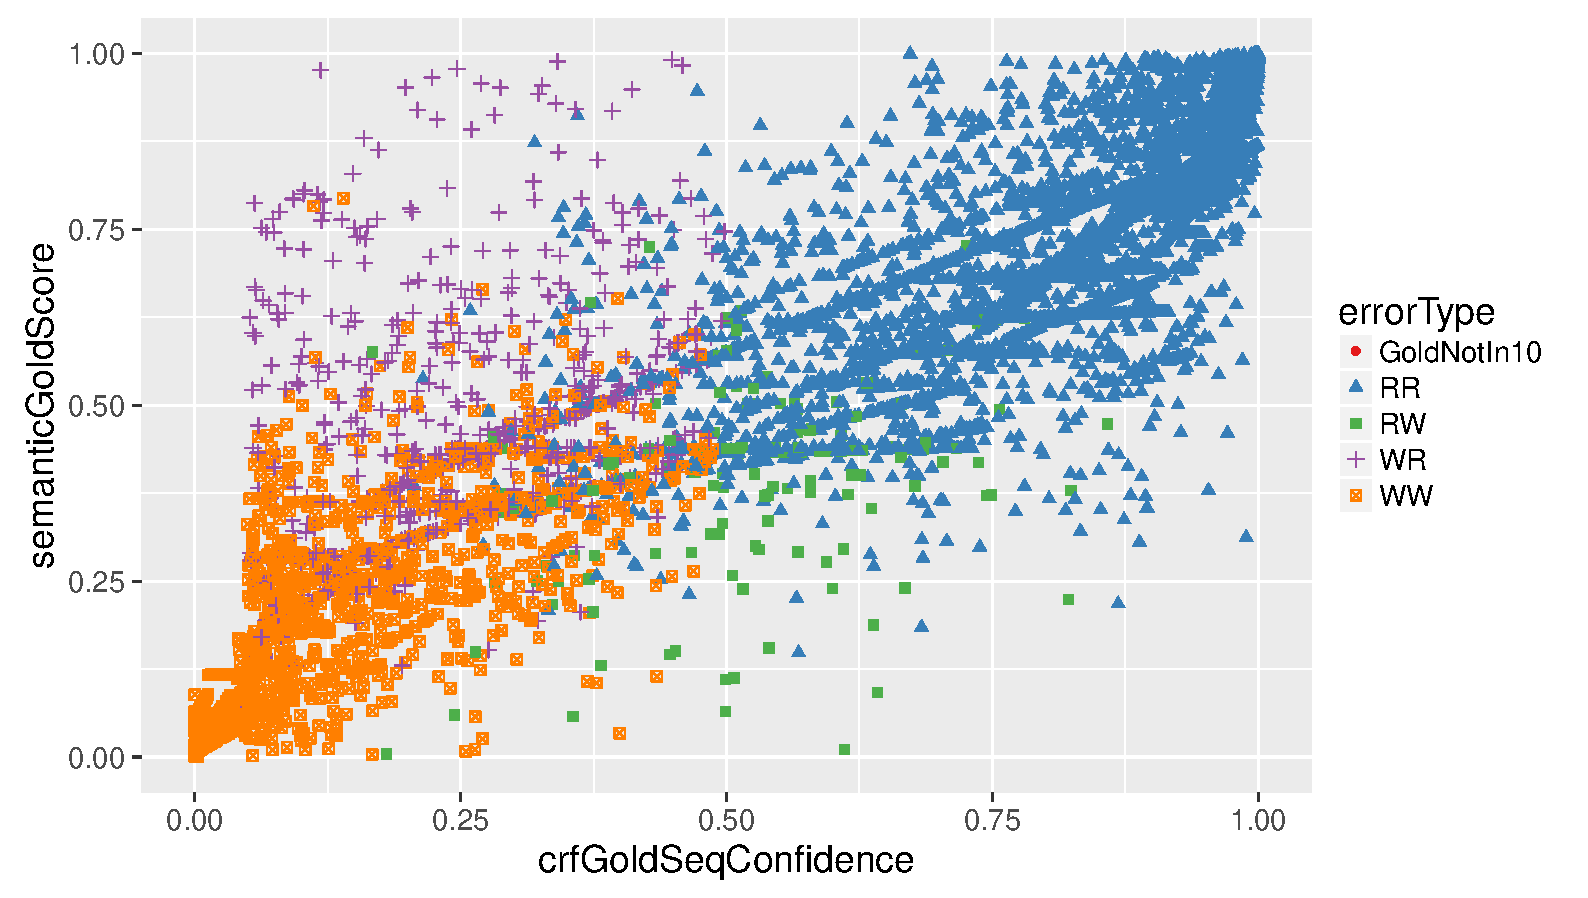
\includegraphics[width=\textwidth]{figures/graph-points-gold-confidence-vs-score-by-error-type.pdf}}
      {\caption{{ Reranker score w.r.t CRF confidence for the gold
            sequence in every sentence, by error type (all languages
            together).} A sentence is represented in the right half
          (resp. left half) if the CRF assigned a high confidence
          (resp. low) to its gold sequence, i.e. the CRF answer is
          correct (resp. incorrect). Similarly, a sentence appears in
          the top half (resp. bottom half) if the reranker assigned a
          high score (resp. low) to its gold sequence, i.e. the
          reranker answer is correct
          (resp. incorrect).\protect\footnotemark
        }\label{fig:goldConfidenceVsScoreByError}} 
\end{figure}


\footnotetext{Remark: Category {\em GoldNotIn10} is not visible on
  this graph, since in such cases the gold sequence cannot be assigned
  a CRF confidence nor a reranker score.}



\figref{fig:goldConfidenceVsScoreByError} gives an overview of how
the reranker\is{reranking} improves performance over the CRF predictions. Every
point in this graph represents a sentence, positioned according to the
CRF confidence (X axis) and reranker final score (Y axis) for its gold
sequence. This way, if the CRF finds the right answer for a sentence,
i.e. the gold sequence obtains the highest confidence among the 10
sequences, it is represented in the right half of the graph, and
conversely for wrong answers. If the reranker finds the right answer,
it assigns a high score to the gold sequence, so the sentence appears
in the top half, and conversely. This explains why the four error
types appear mostly clustered each in its own quadrant: the top right
quadrant contains sentences for which the correct sequence is
recognized by both the CRF and the reranker (hence in the {\it RR}
error category), and the bottom left contains sentences for which
neither finds the right answer ({\it WW}). The last two quadrants are
the interesting ones, since this is where the reranker changes the CRF
prediction to another sequence: in the top left quadrant, the {\it WR} points
correspond to successful changes, whereas the {\it RW} cases, in the
bottom right quadrant, correspond to mistakes introduced by the
reranker.\footnote{This graph can give the impression that one could
  easily prevent {\it RW} mistakes (bottom right quadrant) by
  accepting any CRF answer with high confidence, but this is due to
  the fact that only the gold sequence is represented here. Thus, for
  cases where the gold sequence has low confidence, some other (wrong)
  sequence has high confidence. Therefore selecting the highest
  confidence sequence would simply prevent any \isi{reranking} to happen, in
  particular for the CRF mistakes which can be fixed.} It can be
observed that the former category outnumbers the latter, thus
confirming the positive contribution of the reranker.
%: more right sequences than wrong ones are reranked as the final prediction.





\subsection{Insight: what the reranker actually does}

The vast majority of the sentences (85.3\% of a dataset in average)
fall into the {\em RR} category, i.e. the reranker simply confirms the
correct CRF answer. The {\em WW} cases account for 7.6\% of the sentences, and
the {\em GoldNotIn10} cases for 4.4\%. The reranker actually changes
only 2.7\% of the answers, and when it does, it does it correctly
81.5\% of the time (2.2\% {\em WR}, 0.5\% {\em RW}).\is{reranking}




\figref{fig:selectedSeqNo} shows how the positions of the
sequences selected by the reranker are distributed. The reranker
strongly favors top positions for its selected sequence; more
precisely, as the position of the sequence decreases, the number of
sentences for which this position is selected decreases exponentially
(this is why a logarithmic scale is used in
\figref{fig:selectedSeqNo}). This trend is regular from the top position,
which is selected 92.5\% of the time, down to the 9th position,
selected in only two cases.\footnote{The small rebound in position 10
  is not significant, as it represents only 3 cases.} This shows that
increasing the number of candidate sequences supplied by the CRF (10
in all our experiments) would not improve the performance of the
reranker, since it seldom selects a sequence associated with a low CRF
confidence (the importance of the CRF confidence as a feature is shown
more clearly in \sectref{moreau:sec:featuresAnalysis} below). Finally the fact
that the reranker makes more correct changes than mistakes is
confirmed in this graph again, by observing that the number of {\em
  WR} cases is higher or equal than the number of {\em RW} cases at
every position.
\is{reranking}


\begin{figure}
%\begin{SCfigure}
  \centering
      {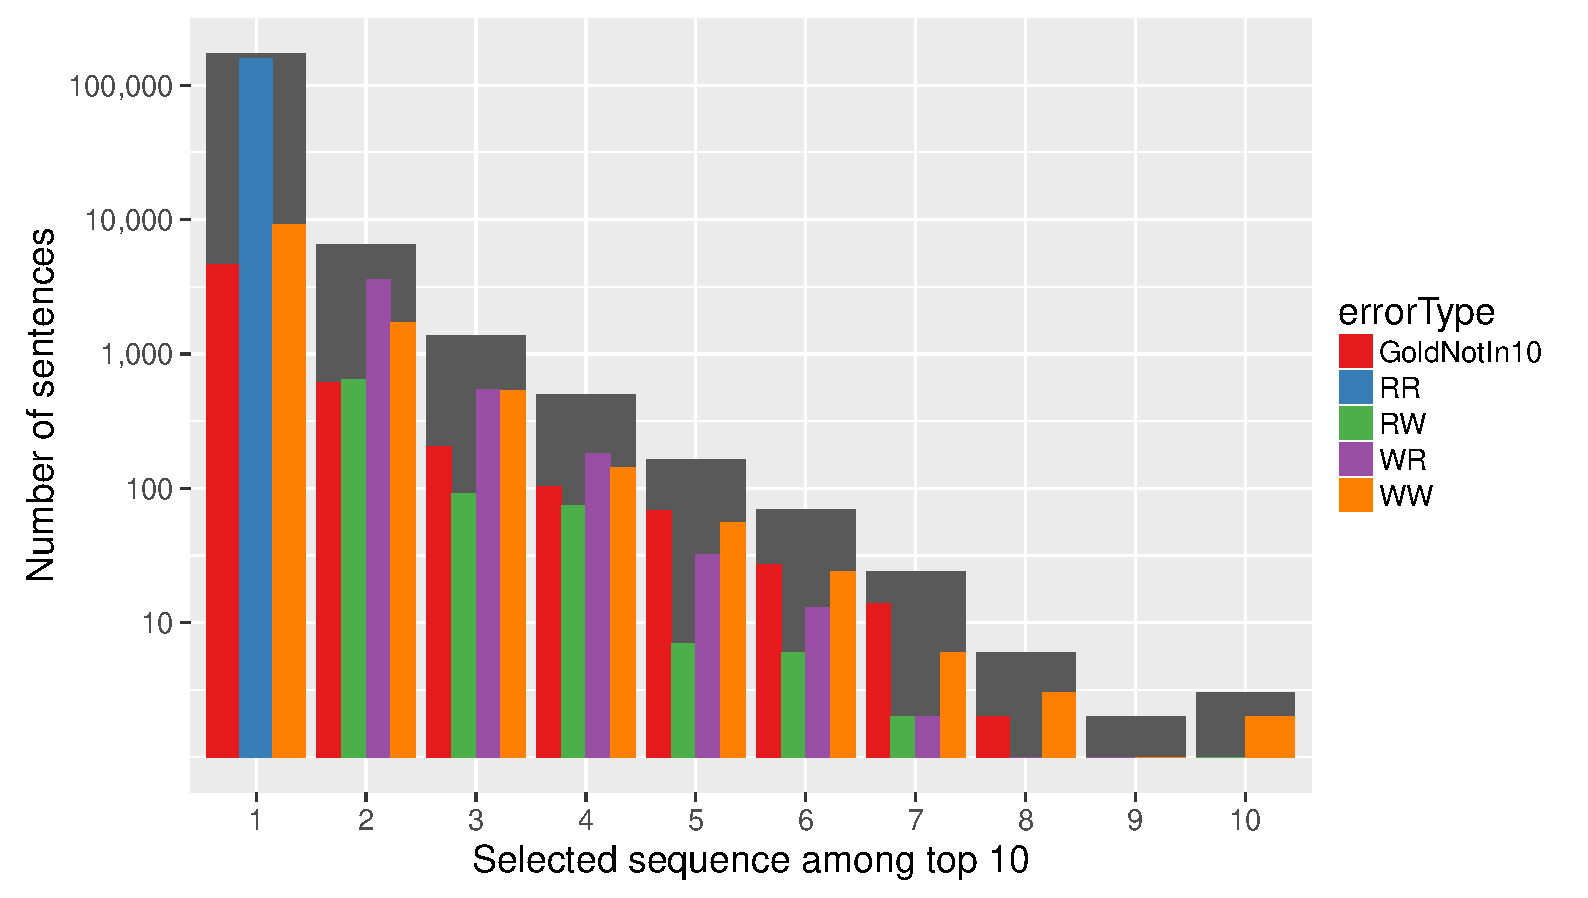
\includegraphics[scale=0.4]{figures/graph-selected-seq-log-by-error-type.pdf}}
      {\caption{{Distribution of the position selected by the reranker
            (logarithmic scale, all languages together).} For every position, the large dark
          grey bar shows the total number of sentences, while the
          coloured bars show the number of sentences for every possible
          error type.\protect\footnotemark
        }\label{fig:selectedSeqNo}}
%\end{SCfigure}
\end{figure}

\footnotetext{This means that the dark grey bar represents the sum of
  the coloured bars, although the logarithmic scale makes this
  difficult to observe. Since the sequence selected by the CRF is the
  top one, position 1 is the only way for both the CRF and the
  reranker answers to be correct, thus it contains all the {\em RR}
  cases. Similarly, it cannot contain any {\em WR} or {\em RW} case,
  by definition.}


  \largerpage
The distribution of errors is not uniform over the data, and the
number of expressions in a sentence is one of the most obvious
factors: For example, \figref{fig:nbExprsByErrorType} shows that
96\% of the sentences with no expression in the gold sequence are
correctly identified by both the CRF and the reranker ({\em RR}),
whereas only 9\% of the sentences with three expressions are. The
difference is mostly due to the proportion of sentences for which the
CRF does not propose the right answer in the top 10 candidate
sequences ({\em GoldNotIn10}), which is naturally higher in the more
complex cases with multiple expressions in the sentence. 
\figref{fig:nbExprsByErrorType} also shows that the reranker is more
useful with the sentences which contain one or two expressions (with
7.4\% and 7.5\% of changes, respectively), because these contain more
mistakes to correct compared to sentences with no expressions, and
contain more possibilities to correct the mistakes compared to
sentences with three (or more) expressions (since the reranker\is{reranking} cannot
correct anything in the {\em GoldNotIn10} cases).
\clearpage 

% ddply(allfeats,'errorType', function(df0) { data.frame(nb=nrow(df0),prop=nrow(df0)/nrow(allfeats))})



% real graph is here:
\begin{figure}
  \scalebox{.35}{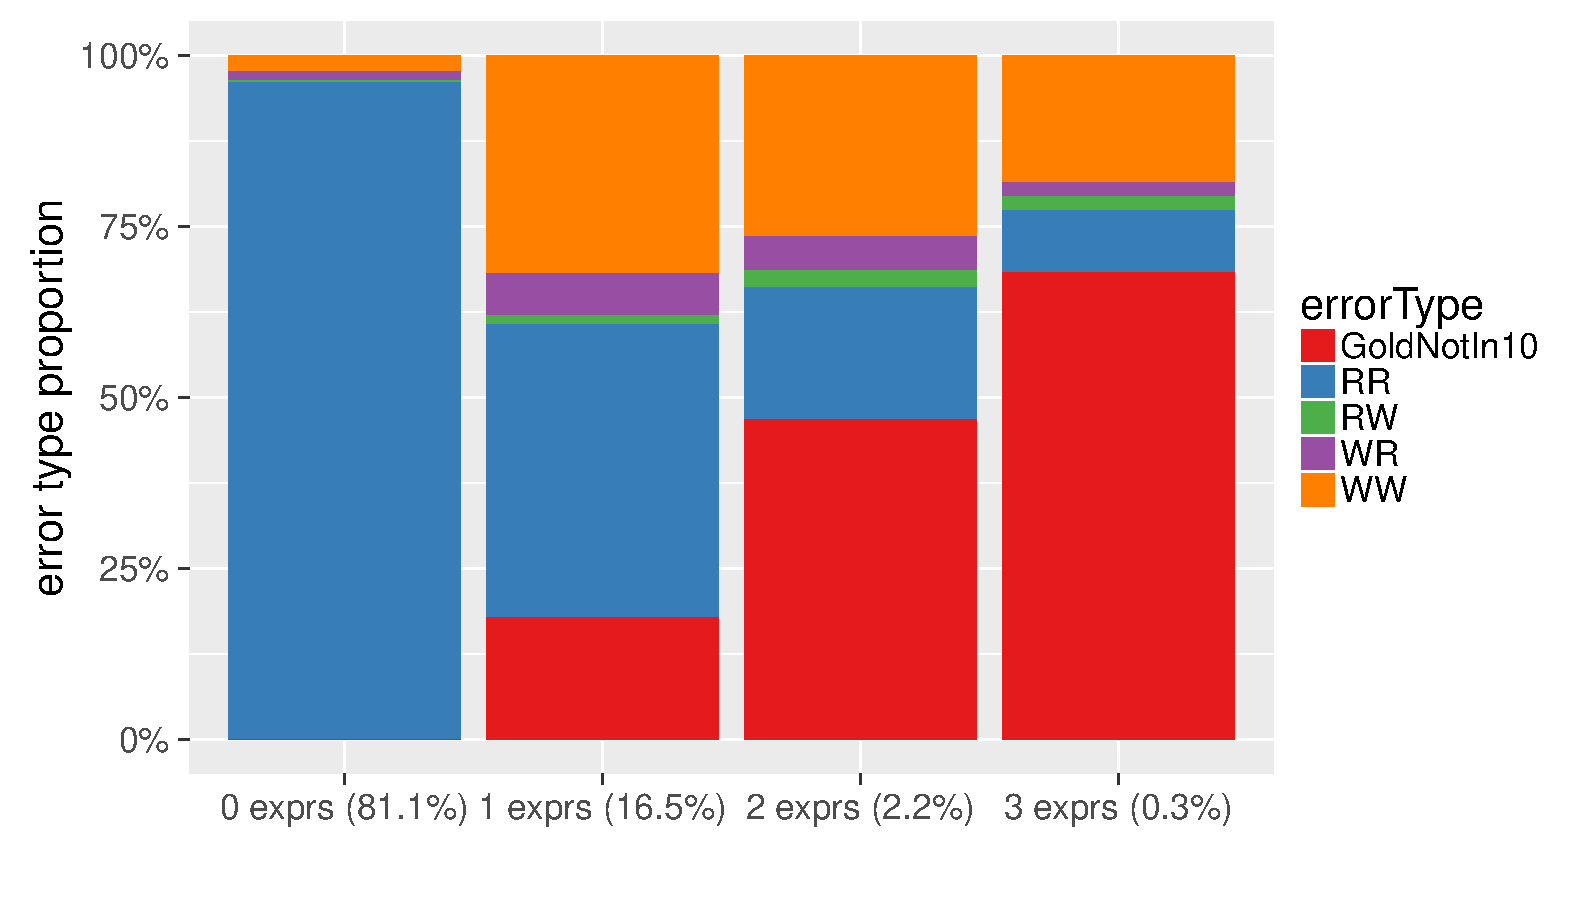
\includegraphics{figures/goldNbExprs0to4ByErrorType-lf.pdf}}
  \caption{{Proportion of error type by number of expressions in the gold sequence (all languages).} Sentences with more than 3 expressions were discarded (30 cases, 0.1\% of the data). Example: 16.5\% of the sentences contain exactly one expression; among these, 18\% belong to the {\em GodNotIn10} category, and 41\%, 1\%, 6\%, 32\% belong respectively to categories {\em RR, RW, WR, WW}. \label{fig:nbExprsByErrorType}}%
\end{figure}

\subsection{Reranker-specific evaluation}
\label{moreau:sec:rerankerEval}


Based on these error types, a new reranker-centered evaluation\is{reranking} method
can be defined. Indeed, using this categorization, the reranker can be
seen as a binary classifier: from this perspective, the job of the
reranker is to detect the sentences for which the CRF answer was
wrong, and leave the right ones as they are. Thus, for every sentence,
either the answer is changed (positive instances) or not (negative
instances). With this idea in mind, the four main categories can be
translated to the standard true/false positive/negative categories in
a straightforward way: if the reranker changes the answer correctly
({\it WR}), the instance is a true positive; if it changes the answer
incorrectly ({\it RW}), the instance is a false positive, and
similarly for the last two cases: {\it RR} and {\it WW} correspond
respectively to true negative and false negative instances (the former
was rightly not changed, and the latter should have been
changed). Thanks to this interpretation, performance measures like
precision, recall and F-score can be calculated for the semantic
reranker, independently from the performance of the CRF
component.\footnote{The {\it GoldNotIn10} category is ignored when
  calculating these performance measures for the reranker,
  consistently with the idea of evaluating the reranker on its own:
  since these cases are impossible to solve, they should not be taken
  into account.} An example of using such performance scores is given
in \tabref{tab:perfNbExprs}.

\begin{table} 
 %   \begin{tabular}{|r|ccc|ccc|}
    \begin{tabularx}{\textwidth}{r@{~~~~}C@{}C@{}C@{~~~~}C@{}C@{}C}
      \lsptoprule

 %   \midrule
%    \multirow{2}{*}{{\scriptsize Nb exprs}} & \multicolumn{3}{c|}{Macro-average} & \multicolumn{3}{c|}{Micro-average} \\
    \multirow{2}{*}{{  Nb exprs}} & \multicolumn{3}{c}{Macro-average} & \multicolumn{3}{c}{Micro-average} \\
                                 & P & R & F & P & R & F \\
 %   \midrule
    \midrule
           0&    82.1&    40.6&    53.8&    83.9&    38.3&    52.6\\
           1&    79.5&    14.5&    23.5&    81.1&    16.1&    26.8\\
           2&    64.3&    20.7&    30.4&    66.0&    15.9&    25.6\\
           3&    75.0&    20.8&    31.0&    50.0&    10.0&    16.7\\
	  \midrule 
         all&    74.9&    18.9&    29.1&    81.4&    22.4&    35.2\\
         %    \midrule
         \lspbottomrule
  \end{tabularx} 
  \caption{{Reranker-specific performance by number of expressions
      in the gold sequence (all languages).} P/R/F stands for
    precision/recall/f-score; the macro-average performance is the
    average over languages (datasets with NaN F-scores are
    ignored).\label{tab:perfNbExprs}}
\end{table}



% is devoted to analyzing the behaviour of the semantic reranker, the results cannot be detailed by dataset
In the rest of this section we do not detail results by dataset, since
the large number of languages and the dataset particularities would
make it harder to recognize the general patterns related to the
reranker.
%, by ``diluting'' them in multiple smaller cases affected by other factors
Nevertheless, it is important to keep in mind that such
dataset-specific factors exist even though they are not
shown. Additionally, the inequal size of the datasets clearly favors
large datasets over small ones when grouping all the sentences
together. This is why we present both the micro-average and
macro-average performance whenever relevant, like in \tabref{tab:perfNbExprs}.


\subsection{Feature analysis}
\label{moreau:sec:featuresAnalysis}


As explained in \sectref{subsec:Sem}, the reranker\is{reranking} uses various kinds of
features to determine the likelihood of the expressions in a
sequence. \tabref{tab:featuresAnalysis} gives a brief overview of
the impact of the different groups of features on performance,
expressed as the F-score, computed from the micro-average precision
and recall of the reranker alone (column 1, see
\sectref{moreau:sec:rerankerEval}), macro-average of the same over languages
(column 2) and expression-level F-score (column 3, official evaluation
on the full system).

First, it should be observed that the reranker relies heavily on the
CRF confidence to make its decisions: without this feature, the
performance drops to a ridiculously low level. Nevertheless, the
reranker needs additional features in order to improve over the CRF
alone (since otherwise the best it can do is to always agree with the
CRF top prediction). A few simple features allow a large gain in performance ({\em SF} in 
\tabref{tab:featuresAnalysis}: number of candidate expressions in the
sequence, min./mean/max. number of words by expression and frequency
in the reference corpus). Adding more
complex features based on frequency and semantic similarity of the
candidate expression allows the reranker to make even better decisions:
the micro F-score reaches 35.6 with the best combination, compared to
32.0 with only {\em SF}. Among these features, frequency and semantic
similarity features seem to be equally useful, and combining both of them
achieves the best performance; the only group of features which
performs poorly (and is apparently even counter-productive) is the one
where the candidate expression is compared against all
other candidates in the sentence (group III in
\tabref{tab:featuresAnalysis}).


\begin{table}
%\begin{SCtable} 
%  \begin{tabular}{|c|c|c|c|}
\fittable{
  \begin{tabular}{l@{}rrr}
          \lsptoprule

%    \midrule
Features       & \parbox{22mm}{\raggedleft micro F-score  reranker}    & 
			\parbox{22mm}{\raggedleft macro F-score reranker}    &
				\parbox{22mm}{\raggedleft macro F-score MWE-level} \\ 
\midrule
\textit{baseline: CRF answer}                    &    NaN   &   NaN    &   48.2    \\
all but confidence                            &   00.6   &   NaN    &   09.6    \\
confidence + SF (*)                           &   32.0   &   NaN    &   53.1    \\
(*) + Ia, Ib                                  &   34.9   &  29.7    &   53.4    \\
(*) + IIa, IIb                                &   34.3   &  29.0    &   53.4    \\
(*) + IIIa, IIIb                              &   33.2   &  27.8    &   53.6    \\
(*) +  IIa, IIb, IIIa, IIIb                   &   34.4   &  29.1    &   53.7    \\
(*) +  Ia, Ib, IIIa, IIIb                     &   34.2   &  29.0    &   53.4    \\
(*) +  Ia, Ib, IIa, IIb                       &{\bf 35.6}&{\bf 30.2}&   53.7    \\
freq. only: (*) + Ia, IIa, IIIa               &   33.9   &  28.7    &   53.7    \\
sem. sim. only: (*) + Ib, IIb, IIIb           &   34.0   &  28.4    &   53.7    \\
all features, with mean only                  &   34.8   &  29.3    &   53.6    \\
all features, with min/mean/max               &   35.2   &  30.1    &{\bf 53.9} \\
%\midrule
\lspbottomrule
  \end{tabular} 
  }
\caption{{ Performance of the reranker using various subsets of
    features (percentages).} Simple features {\em (SF)} represents
  the number of expressions and words as well as the frequency in the
  reference corpus; Groups {\em I}, {\em II} and {\em III} represent
  respectively {\em single word}, {\em expression minus one word} and
  {\em alternative expressions features}; Groups {\em a} and {\em b}
  represent respectively frequency features and semantic similarity
  features (see \sectref{subsec:Sem}); NaN values correspond to cases
  where the precision and/or recall is
  zero.\label{tab:featuresAnalysis}}
%\end{SCtable}
\end{table}


\subsection{Analysis: impact of the coverage in the reference corpus}

Some candidate expressions might not be found in the reference corpus,\is{reranking}
either because they are simply rare or because of
tokenization/lemmatization issues (see \sectref{subsec:europarl}).\is{Europarl corpus} In
fact, the coverage rate of the expressions in Europarl is quite low:
for 36.2\% of the sentences containing at least one expression, the
expression(s) they contain are not found at all in the reference
corpus. \figref{fig:coverage} shows that the error type depends
greatly on whether the expression appears in the reference corpus or
not. First, the CRF finds the right answer much more often when the
expression is covered ({\em RR} + {\em RW} = 73\%) than when it is not
({\em RR} + {\em RW} = 30\%). This can be explained by the fact that
the least frequent expressions are hard to identify by the CRF, and
they also tend not to appear in the reference corpus. While this
implies that the reranker has potentially more mistakes to fix in the
zero-coverage cases, it actually changes fewer sentences (4.4\% against
12.5\% for covered expressions), resulting in a very low recall (3.5\%
against 37.7\%); the precision is also lower, with 67\% against 81\%.

As explained in \sectref{moreau:sec:featuresAnalysis}, the reranker can work
with only a small set of ``simple features'', which is why its
performance in the zero-coverage case is lower but positive. Clearly,
the more advanced features which rely on the reference corpus increase
performance. This means that the coverage in the reference corpus is
critical for the reranker to give its best results, but our current
implementation of the system is probably not optimized from this point
of view; in particular, the tokenization process might not be
identical between the input data (where tokenization is provided) and
the reference data (for which we apply a generic tokenizer), and the
reference corpus is not lemmatized (see \sectref{subsec:europarl}). This
might explain why the recall is low with the current
implementation. Ideally, a larger corpus would also help by covering a
broader range of expressions; but there are very few such large
datasets available for multiple languages.

\begin{figure}
  \scalebox{0.35}{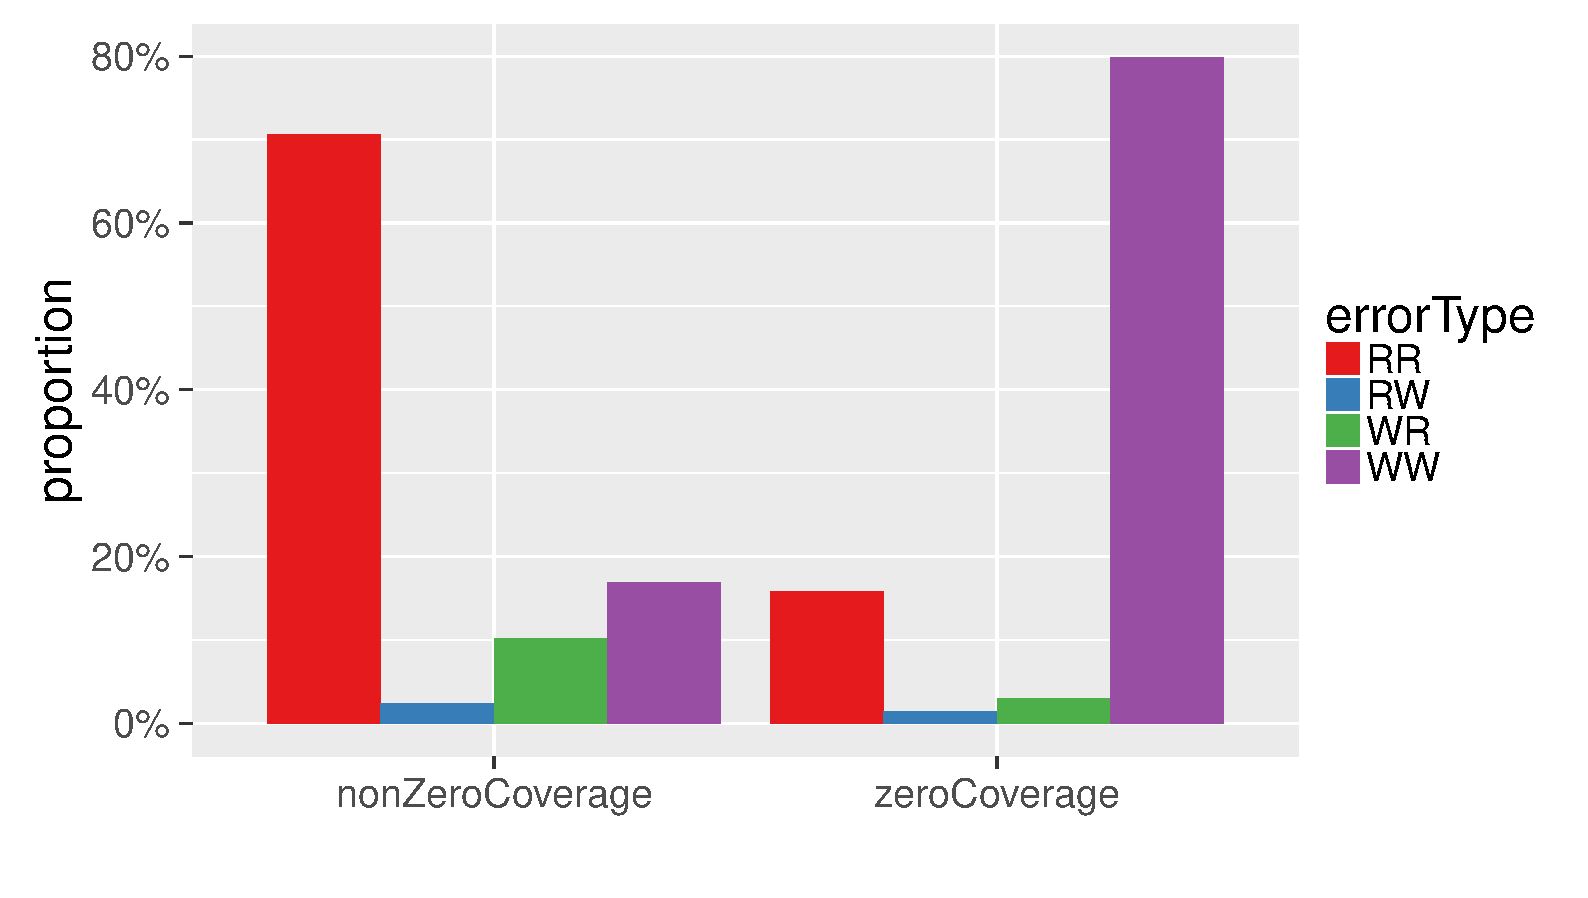
\includegraphics{figures/graph-coverage-ref-corpus-by-error-type.pdf}}
  \caption{{Sentences error types by coverage/non-coverage of
      their expressions in the reference corpus (all languages).}  Example: 70\% of
    the sentences containing expressions which appear in the reference
    corpus belong to the {\em RR} category, whereas only 16\% of the
    sentences with expressions not covered in the reference corpus
    belong to this category.\label{fig:coverage}}
\end{figure}


\subsection{Analysis: continuous vs. discontinuous expressions}
\label{analysisContig}

Verbal multiword expressions can be classified as either continuous
or discontinuous: in the former case, the expression appears as a sequence of
contiguous words, as in the following idiomatic expression:

\vspace*{.2cm}

\begin{minipage}{\linewidth}
\ea 
\langinfo{French}{Indo-European}{FR training data}\\
\gll Celles-ci peuvent à tout moment jeter l' éponge.\\
     they.\textsc{3.fem.pl} can at any time throw the sponge\\
\glt `They.\textsc{3.fem.pl} can give up at any time.'\\
\z
\end{minipage}\\
\\



In the latter case, the expression appears with words
inserted between its lexicalized components, e.g.:

\vspace*{.2cm}

\begin{minipage}{\linewidth}
\ea 
\langinfo{French}{Indo-European}{FR training data}\\
\gll  J'ai \lex{obtenu} de Jean-Marie Molitor [...] \lex{la} \lex{permission} de publier.\\
{I  have} obtained from Jean-Marie Molitor [...] the permission to publish\\
\glt `Jean-Marie Molitor gave me the permission to publish.'\\
\z
\end{minipage}\\
\\


It is worth noticing the same lexicalized components might appear sometimes as
a continuous expression and other times as a discontinuous expression.


\begin{figure}
  \scalebox{0.4}{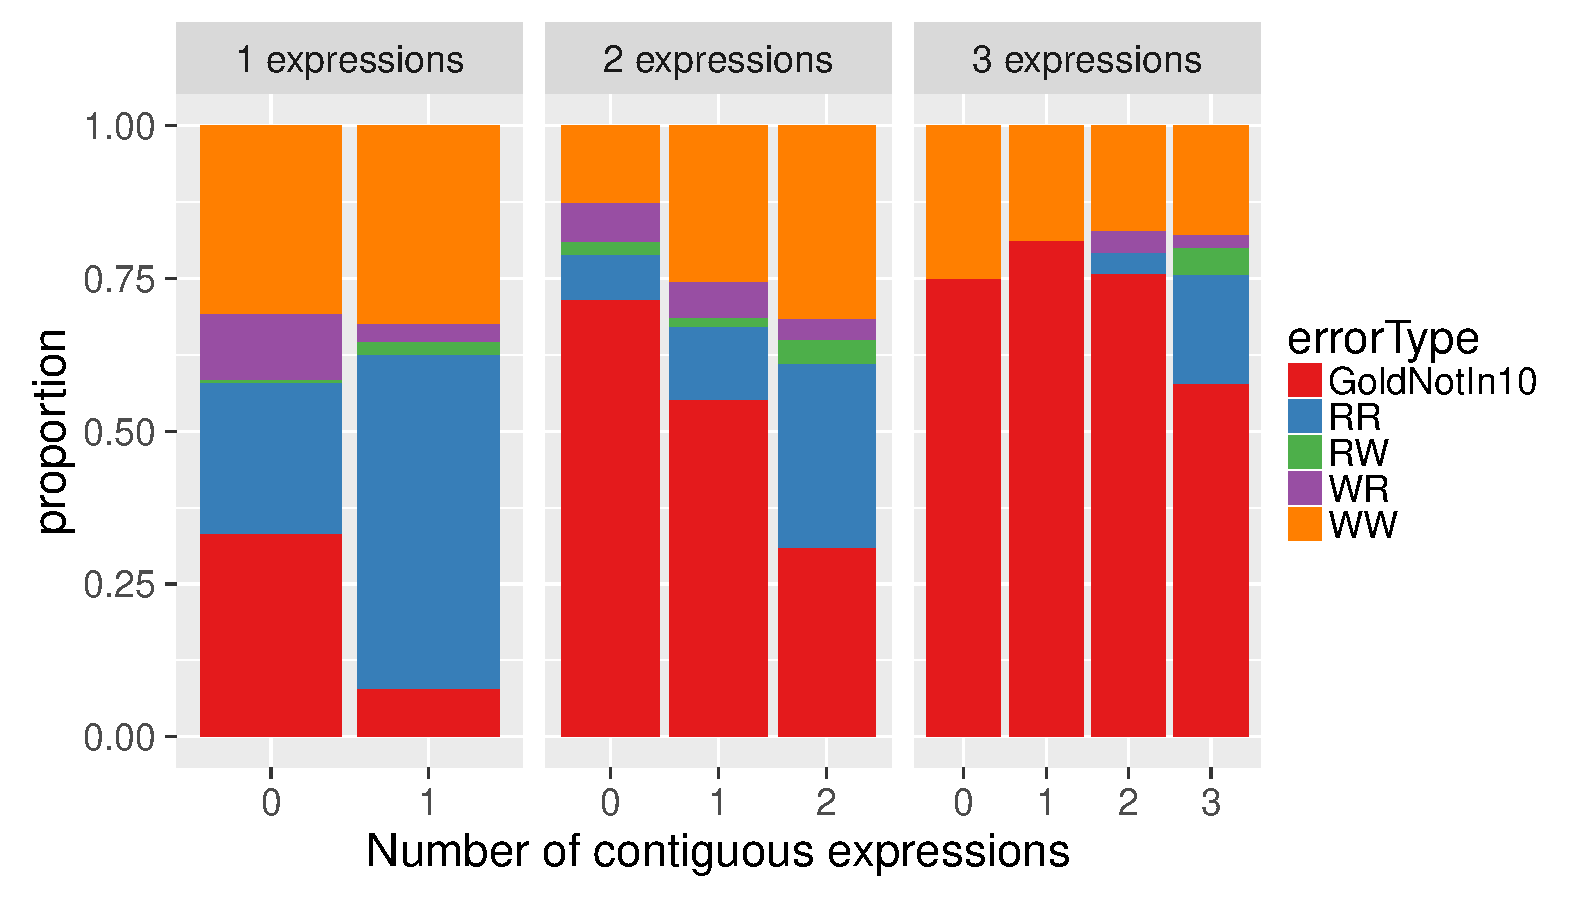
\includegraphics{figures/graph-continuous-nb-exprs.pdf}}
  \caption{{ Proportion of error type by number of continuous
      expressions in the sentence,} for sentences containing 1, 2 or 3
    expressions (all languages). Example: among sentences which contain two
    expressions, the proportion of {\em RR} cases is 7\% (respectively
    12\%, 30\%), when there are no (resp. 1, 2) continuous expressions
    among the two. \label{fig:continuousAnalysis}}
\end{figure}

\clearpage

\figref{fig:continuousAnalysis} shows the impact of continuity\is{multiword expression!continuity} in
expressions: {\em RR+RW} cases increase with the number of continuous
expressions for any number of expressions in the sentence, which means that the more
there are continuous expressions, the better the performance of the
CRF (there are also much less {\em GoldNotIn10} cases). Interestingly,
however, the semantic reranker follows an opposite trend: the less
there are continuous expressions (i.e. the more there are
discontinuous expressions), the better its performance: not only it
fixes more mistakes from the CRF (better recall), it also fixes them
better (better precision).\footnote{Except in the case of three
  expressions with zero or one continuous; this is probably due to the
  low number of cases.} The most likely explanation for these
observations is that the CRF suffers from a ``sequential bias'' which
makes it less good with discontinuous expressions, whereas such cases
are not any harder for the semantic reranker, which is
``sequence-agnostic''. In our opinion, this point clearly illustrates
the complementarity of the two components.



\subsection{Analysis: context vectors options}
\label{analysisContextOptions}


\begin{table}[b]
  \begin{minipage}{.45\linewidth}
    {\centering
    \scalebox{.8}{
  \begin{tabular}{cccccc}
       \lsptoprule
%      \midrule
    \multicolumn{3}{c}{Options} & \multicolumn{3}{c}{Micro-average}\\
    CN & IWIE & MO & P & R & F \\
      \midrule
%    \midrule
      0  &  0  & 0  &  82.9 &   21.9 &   34.6\\
      0  &  0  & 1  &  81.7 &   {\bf 22.4} & {\bf  35.2}\\
      0  &  1  & 0  &  82.5 &   22.1 &   34.8\\
      0  &  1  & 1  &  81.6 &   21.7 &   34.3\\
      1  &  0  & 0  & {\bf 83.3} &   21.8 &   34.5\\
      1  &  0  & 1  &  82.8 &   21.7 &   34.4\\
      1  &  1  & 0  &  80.9 &   21.8 &   34.4\\
      1  &  1  & 1  &  81.4 &   {\bf 22.4} &   {\bf 35.2}\\
%      \midrule 
      \lspbottomrule
  \end{tabular}
    }
    }
  \end{minipage}
  \begin{minipage}{.54\linewidth}
    {\centering
    \scalebox{.8}{
    \begin{tabular}{ccccc}
       \lsptoprule
%     \midrule
      \multicolumn{3}{c}{Options} & {F-score}& F-score\\
      CN & IWIE & MO & {\small Continuous} & {\small Discontinuous}\\
      \midrule
  %    \midrule
      0&    0 &  0 &   14.7 &  {\bf 41.4}\\
      0&    0 &  1 &   {\bf 16.8} &  40.3\\
      0&    1 &  0 &   14.7 &  40.9\\
      0&    1 &  1 &   15.9 &  39.6\\
      1&    0 &  0 &   15.2 &  39.8\\
      1&    0 &  1 &   15.2 &  39.6\\
      1&    1 &  0 &   14.0 &  41.0\\
      1&    1 &  1 &   14.8 &  40.8\\
      \lspbottomrule
      %\midrule 
    \end{tabular}
    }
    }
  \end{minipage}
  
  \caption{{ Performance of the reranker depending on context
      vector options. Left: Overall micro-average performance; right:
      F-score for continuous/discontinuous cases, for sentences with
      one expression exactly.}  CN, IWIE and MO represent the options
    presented in \sectref{subsec:semanticsApproach}, respectively: {\em
      ContextNormalization, IncludeWordsInExpression,
      MultipleOccurrences}.  P/R/F stands for
    precision/recall/f-score. \label{tab:windowOptions}}
\end{table}

In \sectref{subsec:semanticsApproach}, we presented several options
which modify the way words which co-occur with the expression are
taken into account in the MWE \isi{context vector}. 
\tabref{tab:windowOptions} shows the impact on performance of these
options. Although there is no decisive pattern in these results, the
absence of context-level normalization (CN) as well as allowing
multiple occurrences of the same word to be counted multiple times
(MO) obtain slightly higher performance in general. Looking at the
effect of these options on continuous/discontinuous expressions,\is{multiword expression!continuity}
including expressions words in the context window (IWIE) has a
negative effect on all the cases, except if CN is selected but only in
the discontinuous case. In fact, an interesting pattern can be
observed in the continuous/discontinuous table: the combinations of
options which make the F-score increase for continuous expressions
tend to make the F-score in the discontinuous case decrease, and
conversely. This is confirmed by a moderate negative Pearson's
correlation coefficient of -0.56 and a high negative Spearman's rank
correlation coefficient of -0.79. Here again the differences in
performance are too moderate to conclude decisively; however this
point suggests that there is a trade-off between the continuous and
discontinuous cases, and this trade-off might be controlled through
these options to some extent. This means that the system could
potentially be tuned to favor one or the other case.


% despite quite thorough exploration results are not very clear, differences are small
% could be worth including, but lack of time + already too many pages = not worth it
%
% conclusion = goes to future work
%





%% The ``\%" column under ``PS" (henceforth PS\%), in \tabref{tab:Results}, shows the proportion of MWE instances found in the test set that occurred at least once in the training set, i.e. they are ``Previously Seen" MWEs. It is reasonable to expect that most systems would benefit from having a large number of previously seen MWEs in the test set. Our systems tend to perform well when PS\% is high (e.g. \ili{Farsi}, \ili{Romanian}) and poorly when PS\% is low (e.g. \ili{Swedish}), although not in all cases. In fact, this is a trend observed in the other competing systems: the Pearson correlation coefficient between PS\% and all official systems' scores is 0.63. It would indeed be interesting to re-run the competition using a test set that featured MWEs not present in the training set.

%% PS could be potentially regarded as a baseline system that simply attempts to find matches of training MWEs in the test set. Such a simple lookup system, which could compete in the Closed Track, would achieve very high scores in several languages. In fact, it would beat all other systems in the competition in most languages. PS\% can be interpreted as its Recall score. Since such a lookup system is incapable of ``predicting" MWEs it has not seen, we assume it would always achieve a 100\% Precision score, allowing us to compute an F1 score, presented in the ``F1" column in \tabref{tab:Results}, for the baseline PS system.  \tabref{tab:Ranks} shows the number of languages in which each system would rank at each position if we include PS and our unofficial Semantic Re-Ranker scores. Only the 15 languages we attempted are counted. PS would always rank first except only in \ili{French} and \ili{Swedish}, the two languages with the lowest proportion of previously seen MWEs. One might contest PS's 100\% Precision assumption as it depends on the accuracy of the actual VMWE matching method used. However, under this assumption PSF1 measures the best performing lookup method possible. This reasoning feeds into the simple matching method used: VMWEs are extracted from training and test set files according to their gold standard. PS\% is their intersection divided by the total number of test set VMWEs. A VMWE is deemed to be present in both portions if its extracted \isi{dependency} structure (if provided), lemmas and POS tags are identical in both files. For languages without dependencies, MWEs are matched based on lemmas and POS linear sequences only. 

%\begin{table}
%\caption{\label{tab:Ranks}Number of languages each system ranked at. Systems in grey italics are %open systems, the rest are closed. PS and sem are unofficial systems.}
%\centering{}\includegraphics[scale=0.8]{proportions-vs-official-results.pdf}\vspace{-1 em}
%\end{table}

%Interesting questions about the \isi{shared task}'s F1-based evaluation can also be raised. F1 considers Precision and Recall to be equally important, when in reality their relative importance depends on the purpose of an actual VMWE \isi{identification} exercise. In a human-mediated lexicographic exercise, for example, where coverage is more important than avoiding false positives, Recall will take precedence. Conversely, in a computer-assisted \isi{language learning} application concerned with obtaining a small but illustrative list of VMWE examples, Precision will take priority. We suggest that for future iterations of the \isi{shared task}, a few candidate applications be identified and subtasks be organised around them. The \isi{identification} task's purpose will also inform on the appropriateness of including previously seen MWEs in the test set. In a lexicographic or terminological task, there is usually an interest in identifying \emph{new}, \emph{unseen} MWEs as opposed to \emph{known} ones, whereas in Machine Translation, the impact of known MWEs in new, \isi{unseen} sentences is of interest.

\section{\label{moreau:sec:conc2}Conclusion and future work}


In this chapter we described a two stages approach for identifying
VMWEs, based on sequence labeling with CRF followed by \isi{reranking} of
the CRF candidates. We showed experimentally that the reranker
significantly improves the performance of the system, with in average
a 12\% F1-score improvement over using the CRF component alone. Then
we proceeded to analyze how the reranker works.

We found that the reranker follows the CRF quite closely, rarely
selecting a candidate with a low CRF confidence, and selecting the CRF
top prediction in 92.5\% of the cases. Consistently with this
observation, when the reranker diverges from the top CRF prediction,
it does so correctly with high confidence (81.5\% of correct answers
among the changed predictions).

The contribution of the reranker is more important with the sentences
which contain one or two expressions: sentences with no expressions
are almost always correctly detected by the CRF alone, whereas the
cases with 3 or more expressions are so complex that the CRF does not
usually provide the right candidate among its top 10 predictions,
leaving the reranker unable to fix these errors. The coverage of the
MWE in the reference corpus is another major factor of performance for
the reranker, with the recall dropping 10 times for expressions which
do not appear in the reference corpus. Finally the last important
finding of our study is that the reranker seems to compensate the CRF
sequential bias: while the latter performs better with continuous
MWEs, the reranker performs comparatively better with discontinuous
cases.\is{multiword expression!continuity}

The semantic reranker presented in this chapter is a proof-of-concept
version, and new perspectives emerge from the fact that the
combination of a CRF component with this reranker proves fruitful for
detecting MWEs. There are a few obvious areas in which the reranker
could be improved, especially in the tokenization/lemmatization part,
and it is likely that choosing a more adequate reference corpus would
help. But there are also deeper questions which are worth studying:

\begin{itemize}
\item Computing a \isi{context vector} for a MWE is not as trivial as for a
  single word (especially if the words in the expression are not
  continuous), and the authors are not aware of any standard approach
  for this. While several options were tested, this question deserves
  to be studied on its own.
\item In the same line of thought, the current state of the art in
  \isi{distributional semantics} is based on \isi{word embeddings}
  \citep{legrand2016phrase}. Here again, the authors are not
  aware of any software able to retrieve word embeddings for multiple
  (possibly discontinuous) words.
\item Would it be possible for the reranker to work at the expression
  level instead of the sentence level? Indeed, the current method used
  to ``merge'' multiple expressions in a sentence is likely to lose
  some information in the process. One could also ask whether some of
  the information currently computed by the reranker could be fed directly
  into the CRF. An iterative process could even be considered, perhaps
  allowing to refine the quality of the predicted expressions over
  iterations.
\end{itemize}



%In this paper, we described our VMWE \isi{identification} systems based on CRF and Semantic \isi{reranking}, achieving competitive results. Our future work will focus on language-specific features, rather than on language families. We also intend to explore tree-based CRF methods to better exploit syntactic \isi{dependency} tree structures. The promising first results obtained with the Semantic Reranker deserve to be explored further. Aspects such as parameter tuning, feature selection and other semantic vector types, like \isi{word embeddings},  might help improve the performance. Finally, we want to explore alternative evaluation methods based on lexicographic and terminological tasks \citep{Maldonado2016} on the one hand and Machine Translation tasks \citep{xiong2016topic} on the other.




%%We analysed the role of previously seen MWEs and showed that they help all systems in the competition, including a hypothetical, simple lookup system that would beat all systems in most languages. We also argued for a more purpose-based evaluation scheme. 



\section*{Acknowledgements}

We are grateful to the editors and anonymous reviewers for their valuable comments. Lifeng Han also thanks Qun Liu for his continued support. 

The ADAPT Centre for Digital Content Technology is funded under the SFI Research Centres Programme (Grant 13/RC/2106) and is co-funded under the European Regional Development Fund.



The graphics in this chapter were created with \texttt{R} \citep{R}, using the \texttt{ggplot2} library \citep{ggplot2}.


\section*{Abbreviations}

   \begin{tabularx}{.48\textwidth}{ll}
    \textsc{crf} & conditional random fields\\
   \textsc{idf}  & inverse document frequency\\  \textsc{mwe}  & multiword expression\\
  \textsc{nlp}  & Natural Language Processing\\
 \textsc{rr}  & right-right\\
      \end{tabularx}
      \begin{tabularx}{.48\textwidth}{ll}
 \textsc{rw}  & right-wrong\\
   \textsc{vmwe}  & verbal mutiword expression\\  \textsc{wr}  & wrong-right\\
  \textsc{ww}  & wrong-wrong\\
  \\
  \end{tabularx}


{\sloppy
\printbibliography[heading=subbibliography,notkeyword=this]
}
\end{document}
